With the magnetic field of 5 T and temperature of ~ 1 K, we expect to obtain polarization 
values of  80-90\% (30-40\%) for the ammonia (deuterated ammonia) targets.
Target polarization will be monitored using the NMR system.
The target cell size in the current design is relatively large, 
which will allow for placement of the NMR coils inside of the cell resulting in a 
measurable thermal equilibrium signal. The polarization of deuterium will be 
monitored  by the area and ratio methods.
Typical NMR signals 
for the proton and deuterium targets are shown in Fig. \ref{nmr}.
The signals are obtained from the small target cells 
with NMR coils wrapped on the ouside, and represent the minimum expected quality.

%%%%%%%%%%%%%%%%%%%%%%%%%%%%%%%%%%%%%%%%%%%%%%%%%%%%%%%%%%%%%%%%%%%%%%%%%%
\begin{figure}
\centering
\begin{minipage}[t]{0.5\linewidth}
\centering
\includegraphics[width=2.45in]{\plots/NH3.eps} 
\end{minipage}%
\begin{minipage}[t]{0.5\linewidth}
\centering
\includegraphics[width=2.45in]{\plots/ND3.eps} 
\end{minipage}
\caption{\small{NMR signals for polarized NH$_3$(left) and ND$_3$(right).}}
\label{nmr}
\end{figure}
%%%%%%%%%%%%%%%%%%%%%%%%%%%%%%%%%%%%%%%%%%%%%%%%%%%%%%%%%%%%%%%%%%%%%%%%%%

Ammonia can accumulate a charge of $\sim 10^{15}$ 
electrons/cm$^2$ before showing signs of deterioration.
 Accumulated radiation damage can be mostly restored through 
the annealing process, in which target material is heated to temperatures of 80-90 K for short periods of time.
At a flux of 9.22 $\times$ 10$^{10}$ electrons/s (14.7 nA), 
a 3 cm diameter target would accumulate a dose of  
$\sim$ 5 $\times$ 10$^{15}$ $e^-/cm^2$ in 4 days (106 hours). 
If ammonia is used as the target material then frequent target anneals and target changes 
should be anticipated. 
Experience with the existing Hall B polarized target has demonstrated that 
withdrawing the target to a heated region, 
rather that attempting to heat the 1K section of the cryostat, is an effective method of annealing the target.  A load lock for the target insert could be useful both for frequent target anneals and changes.
It may also be desirable to increase the diameter in order to extend target lifetime.
A history of target polarization as a function of accumulated charge and anneal cycles 
is shown in Figs.~\ref{raddamage-nh3} and \ref{raddamage-nd3}.

%%%%%%%%%%%%%%%%%%%%%%%%%%%%%%%%%%%%%%%%%%%%%%%%%%%%%%%%%%%%%%%%%%%%%%%%%%
\begin{figure}[h]
\centering
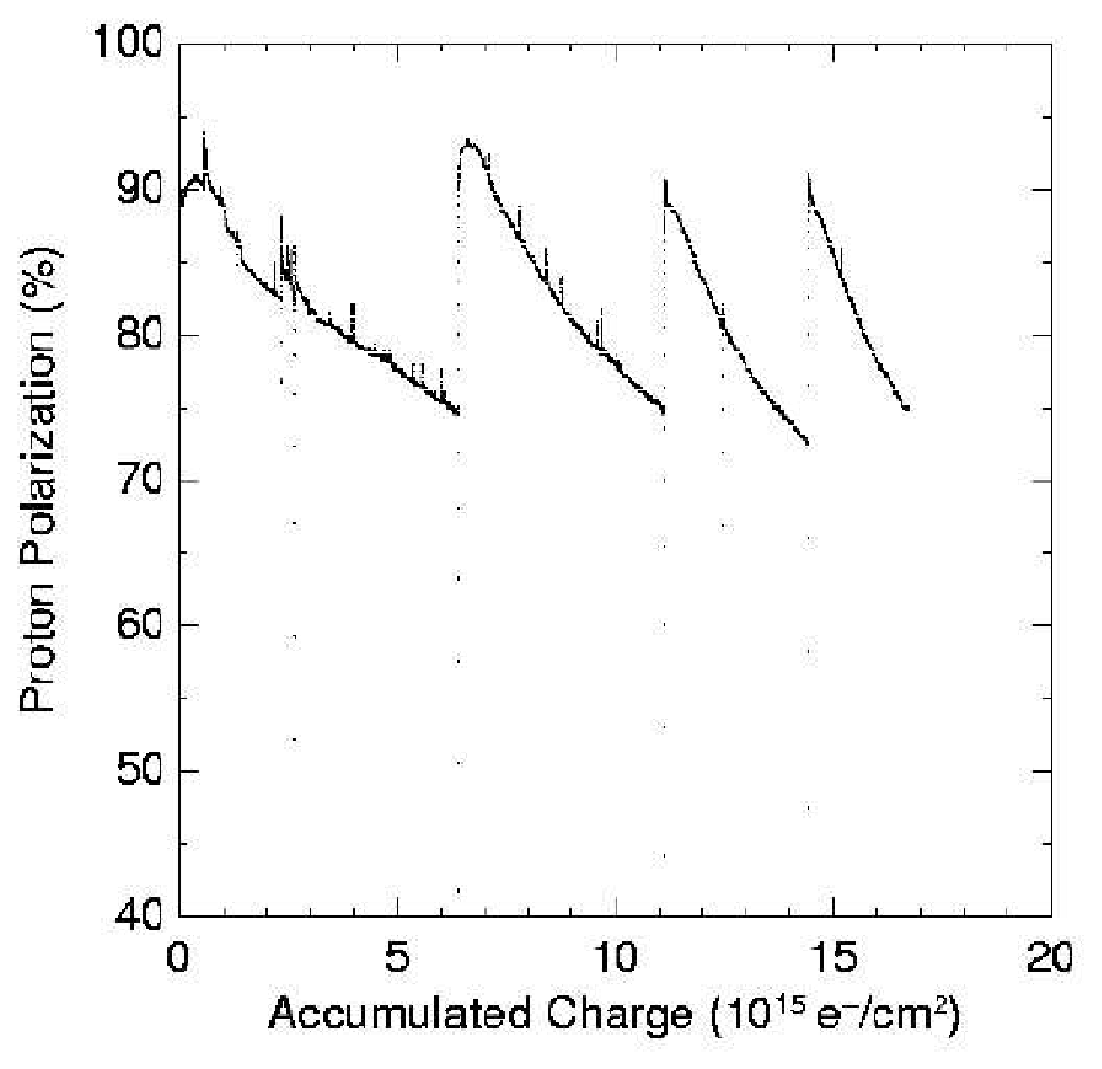
\includegraphics[width=\textwidth]{\plots/nh3_rad_damage.eps}
\caption{\small{$^{15}$NH$_3$ polarization as a function of time.}}
\label{raddamage-nh3}
\end{figure}
%%%%%%%%%%%%%%%%%%%%%%%%%%%%%%%%%%%%%%%%%%%%%%%%%%%%%%%%%%%%%%%%%%%%%%%%%%

%%%%%%%%%%%%%%%%%%%%%%%%%%%%%%%%%%%%%%%%%%%%%%%%%%%%%%%%%%%%%%%%%%%%%%%%%%
\begin{figure}[h]
\centering
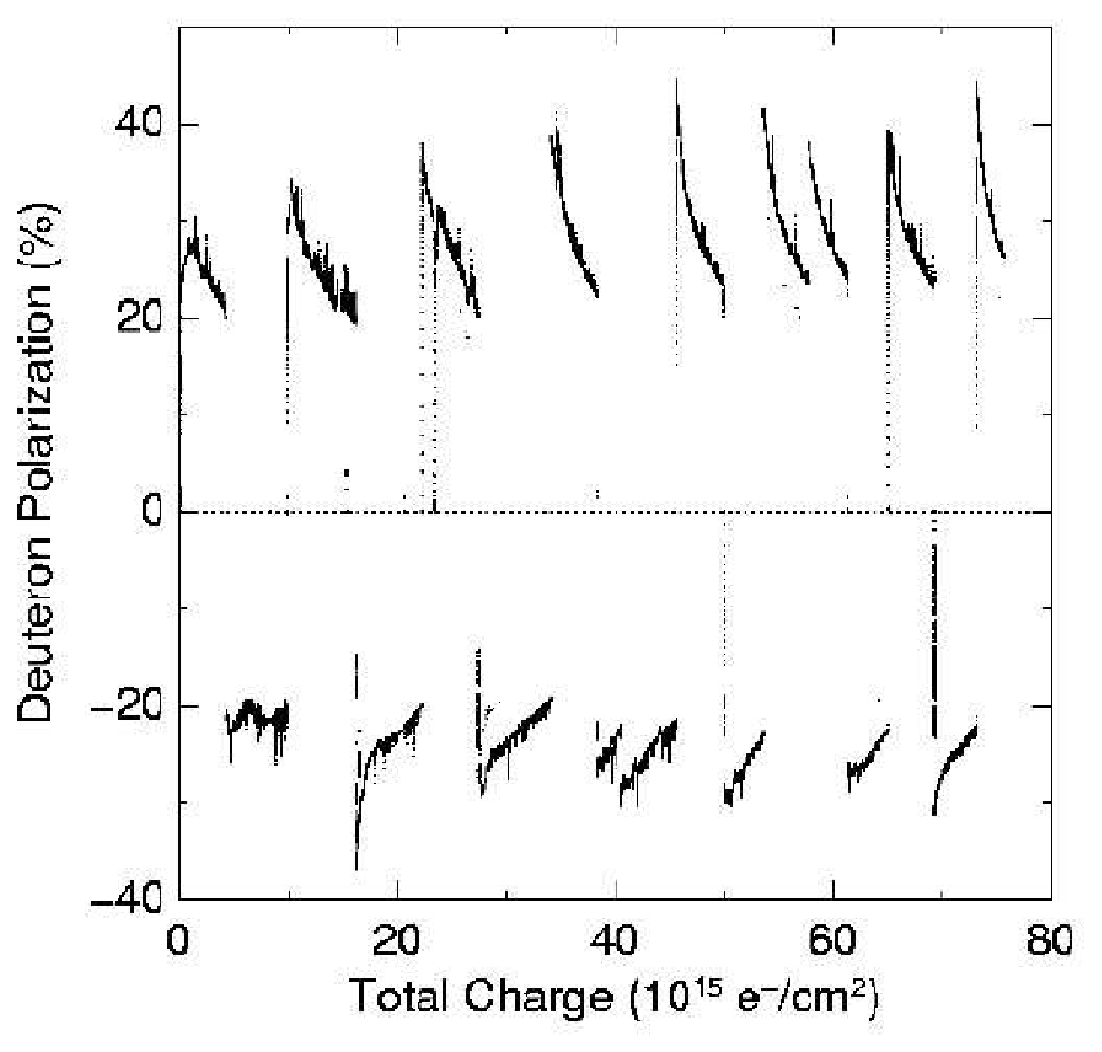
\includegraphics[width=\textwidth]{\plots/nd3_rad_damage.eps}
\caption{\small{$^{15}$ND$_3$ polarization as a function of time.}}
\label {raddamage-nd3}
\end{figure}
%%%%%%%%%%%%%%%%%%%%%%%%%%%%%%%%%%%%%%%%%%%%%%%%%%%%%%%%%%%%%%%%%%%%%%%%%%

